\section{Trasformata di Fourier}

In questa sezione daremo la definizione e richiameremo alcune importanti
proprietà che riguardano la trasformata di Fourier.\\
La trasformata di Fourier viene introdotta per poter dare una rappresentazione
simile a quella fornita dalle serie di Fourier per le funzioni non periodiche.

\begin{definition}
    % TODO: aggiungere ?? f (una funzione che rappresenta un segnale) 
    Sia $f \in L^1(\mathbb{R})$. Allora la trasformata di Fourier di $f$ è
    definita come:

    $$
        \hat{f}(\lambda) := \int_{-\infty}^{+\infty} f(x) e^{-i\lambda x} \ dx,
        \ \lambda \in \mathbb{R}
    $$
\end{definition}

\paragraph{Note:}
\begin{itemize}
    \item Ricordiamo che $e^{-i\lambda x} = \cos(\lambda x) - i \sin(\lambda x)$
    \item Ricordiamo i numeri complessi definiti come:
          \begin{equation}\label{eq:modi}
              z = a + ib
          \end{equation}

          dove $a$ viene detta \textit{parte intera} e $b$ la \textit{parte
              immaginaria}.
    \item Il modulo di un numero complesso è definito come:
          \begin{equation}\label{eq:modi2}
              |z| = \sqrt{a^2 + b^2}
          \end{equation}
          \begin{center}
              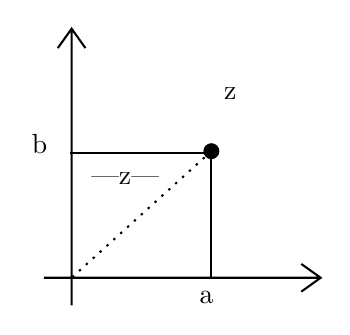
\begin{tikzpicture}[x=1.0pt,y=1.0pt,yscale=-1,xscale=1]
                  %uncomment if require: \path (0,300); %set diagram left start
                  %at 0, and has height of 300

                  %Straight Lines [id:da5730343469684522] 
                  \draw    (150.5,189.75) -- (150.5,234.75) ;
                  %Straight Lines [id:da70665287162995] 
                  \draw    (99.5,189.75) -- (150.5,189.75) ;
                  %Shape: Axis 2D [id:dp7340131235297938] 
                  \draw  (90,235) -- (190,235)(100,145) -- (100,245) (183,230)
                  -- (190,235) -- (183,240) (95,152) -- (100,145) -- (105,152)
                  ;
                  %Shape: Circle [id:dp17035889321633024] 
                  \draw  [fill={rgb, 255:red, 0; green, 0; blue, 0 }  ,fill
                      opacity=1 ] (148,189.25) .. controls (148,187.87) and
                  (149.12,186.75) .. (150.5,186.75) .. controls (151.88,186.75)
                  and (153,187.87) .. (153,189.25) .. controls (153,190.63) and
                  (151.88,191.75) .. (150.5,191.75) .. controls (149.12,191.75)
                  and (148,190.63) .. (148,189.25) -- cycle ;
                  %Straight Lines [id:da11421787184111976] 
                  \draw  [dash pattern={on 0.84pt off 2.51pt}]  (150.5,189.25)
                  -- (100,235) ;

                  % Text Node
                  \draw (154,165) node [anchor=north west][inner sep=0.75pt]
                  [align=left] {z};
                  % Text Node
                  \draw (145,239) node [anchor=north west][inner sep=0.75pt]
                  [align=left] {a};
                  % Text Node
                  \draw (84.5,182) node [anchor=north west][inner sep=0.75pt]
                  [align=left] {b};
                  % Text Node
                  \draw (106,196) node [anchor=north west][inner sep=0.75pt]
                  [align=left] {|z|};


              \end{tikzpicture}
          \end{center}
    \item Quindi
          $$
              |e^{-i \lambda x}| = (\cos^2 (\lambda x) + \sin^2(\lambda
              x))^{\frac{1}{2}} = 1
          $$

\end{itemize}

\vspace{1cm}

Ci domandiamo il perché sia così importante che $f \in L^1(\mathbb{R})$
(possibile domanda di esame).\\

\begin{center}
    Se $f \in L^1(\mathbb{R})$ allora $\hat{f} \in L^1(\mathbb{R})$.
\end{center}

\begin{proof}
    Poiché $f \in L^1(\mathbb{R})$, la funzione $\hat{f}(\lambda)$ risulterà
    sicuramente ben definita, infatti:

    \begin{equation}
        \begin{aligned}
            |\hat{f}(\lambda)| & = \left|\int_{\mathbb{R}} f(t) e^{-i \lambda t} \ dt \right| \leq \int_{\mathbb{R}} |f(t) e^{-i \lambda t}| \ dt =                  \\
                               & = \int_{\mathbb{R}} |f(t)| \cdot |e^{-i \lambda t}| \ dt = \int_{\mathbb{R}} |f(t)| \ dt < + \infty, \forall \lambda \in \mathbb{R}
        \end{aligned}
    \end{equation}

    Risulta essere $< +\infty$ \textit{se e solo se} $f\in L^1(\mathbb{R})$

\end{proof}

%%siamo sicuri di questa cosa ???
Ma, in generale non possiamo affermare che $\hat{f}(\lambda)
    \in L^1(\mathbb{R})$.\\

%% TODO: la successiva parte che riguarda il grafico del segnale non l'ho
%capita.

Ci accorgiamo ora che, nella realtà, molto spesso abbiamo a che fare con segnali
\textit{"in banda"} (espressi con la rispettiva trasformata di Fourier) e
risulterebbe molto comodo poter riuscire a risalire alla funzione originale. In
altre parole ci domandiamo se esiste l'inverso della Trasformata di Fourier.

\begin{theorem}
    Sia $f \in L^1(\mathbb{R}) \cap C^0(\mathbb{R})$ e tale che $\hat{f} \in
        L^1(\mathbb{R})$. Allora definiamo la \textit{Trasformata Inversa di
        Fourier} come:

    $$
        f(x) = \int_{-\infty}^{+\infty} \hat{f}(\lambda) e^{i \lambda x} \
        d\lambda, \ \ \forall x \in \mathbb{R}
    $$
\end{theorem}

\begin{proof}
    Poiché $\hat{f} \in L^1(\mathbb{R})$, la funzione $f(x)$ risulterà
    sicuramente ben definita, infatti:

    \begin{equation}
        \begin{aligned}
            |f(x)| & = \left|\int_{\mathbb{R}} \hat{f}(\lambda) e^{i \lambda t} \ d\lambda \right| \leq \int_{\mathbb{R}} |\hat{f}(\lambda)| \ d\lambda < + \infty, \forall x \in \mathbb{R}
        \end{aligned}
    \end{equation}

    Risulta essere $< +\infty$ \textit{se e solo se} $\hat{f}\in L^1(\mathbb{R})$

\end{proof}

Il precedente Teorema permette di esprimere $f$ in termini della sua Trasformata
di Fourier. Questo rappresenta la Trasformata Inversa di Fourier e possiamo
indicarla anche con $\hat{f}^{-1}$.

\begin{center}

    \tikzset{every picture/.style={line width=0.75pt}}

    \begin{tikzpicture}[x=0.75pt,y=0.75pt,yscale=-1,xscale=1]
        %uncomment if require: \path (0,300); %set diagram left start at 0, and
        %has height of 300

        %Shape: Axis 2D [id:dp5823155267563114] 
        \draw  (88,155.67) -- (188,155.67)(138.33,71) -- (138.33,171)
        (181,150.67) -- (188,155.67) -- (181,160.67) (133.33,78) -- (138.33,71)
        -- (143.33,78)  ;
        %Shape: Axis 2D [id:dp9473219631031637] 
        \draw  (400,155.67) -- (500,155.67)(450.33,71) -- (450.33,171)
        (493,150.67) -- (500,155.67) -- (493,160.67) (445.33,78) -- (450.33,71)
        -- (455.33,78)  ;
        %Curve Lines [id:da9507777176571728] 
        \draw    (90,129) .. controls (130,99) and (150,159) .. (190,129) ;
        %Curve Lines [id:da8695662202477725] 
        \draw    (398.67,142) .. controls (434.33,143) and (436.33,105) ..
        (451,104.33) .. controls (465.67,103.67) and (453.67,141.67) ..
        (498.67,142) ;
        %Curve Lines [id:da04668467081792005] 
        \draw [color={rgb, 255:red, 208; green, 2; blue, 27 }  ,draw opacity=1 ]
        (216.33,69) .. controls (255.13,39.9) and (349.45,46.87) ..
        (374.84,68.3) ; \draw [shift={(377,70.33)}, rotate = 226.71] [fill={rgb,
                    255:red, 208; green, 2; blue, 27 }  ,fill opacity=1 ][line width=0.08]
        [draw opacity=0] (8.93,-4.29) -- (0,0) -- (8.93,4.29) -- cycle    ;
        %Curve Lines [id:da6399644807337441] 
        \draw [color={rgb, 255:red, 208; green, 2; blue, 27 }  ,draw opacity=1 ]
        (220.96,189.96) .. controls (244.28,247.55) and (372.49,228.17) ..
        (380.33,187.67) ; \draw [shift={(219.67,186.33)}, rotate = 72.68]
        [fill={rgb, 255:red, 208; green, 2; blue, 27 }  ,fill opacity=1 ][line
            width=0.08]  [draw opacity=0] (8.93,-4.29) -- (0,0) -- (8.93,4.29) --
        cycle    ;

        % Text Node
        \draw (287.33,56) node [anchor=north west][inner sep=0.75pt]
        [color={rgb, 255:red, 208; green, 2; blue, 27 }  ,opacity=1 ]
        [align=left] {$\displaystyle \hat{f}$};
        % Text Node
        \draw (289.33,191.33) node [anchor=north west][inner sep=0.75pt]
        [color={rgb, 255:red, 208; green, 2; blue, 27 }  ,opacity=1 ]
        [align=left] {$\displaystyle f$};


    \end{tikzpicture}

\end{center}

\paragraph{Note:}
\begin{itemize}
    \item $C^0(\mathbb{R}) = \{ f: \mathbb{R} \rightarrow \mathbb{R} | f \text{
                  risulta continua in } \mathbb{R} \}$. Ovvero, $C^0(\mathbb{R})$ è
          l'insieme di tutte le funzioni che risultano continue in
          $\mathbb{R}$.
\end{itemize}

Analizziamo ora alcune proprietà della Trasformata di Fourier.

\begin{theorem}
    Sia $f \in L^1(\mathbb{R})$, allora la funzione $\hat{f}(\lambda) \in
        C^0(\mathbb{R})$ e vale:

    $$
        \lim_{\lambda \rightarrow +\infty} \left| \hat{f}(\lambda) \right| = 0.
    $$
\end{theorem}

Ricordiamo che le funzioni che sono in $L^1(\mathbb{R})$ non è detto che siano
continue ! Una funzione può essere integrabile anche se ha un numero finito di
punti di discontinuità. Il precedente teorema ci va a dire che se applico la
Trasformata di Fourier ad una funzione che non è continua (ma comunque
integrabile), allora il risultato sarà sicuramente una funzione continua e
che quella funzione sarà integrabile ! Questo è anche visibile dal grafico che
otterremmo in quanto avrà le "code" che si schiacciano su zero.\\
Questa proprietà viene anche chiamata \textit{"Regolarizzazione"}.
%% TODO: c'è anche un secondo significato a questo teorema, ci assicura che %
%all'infinito la funzione tende a 0, ma non so bene spiegarlo. Vanno rivisti gli
%appunti (ci assicura che sia 0 perché se no si schiacciasse l'area sotto la
%funzione tenderebbge a +inf, ed il suo itegrale sarebbe di conseguenza non finito)

\begin{theorem}
    Siano $f, g \in L^1(\mathbb{R})$ e $\alpha, \beta \in \mathbb{C}$ allora:

    $$
        (\widehat{ \alpha f + \beta g })(\lambda) = \alpha \hat{f}(\lambda) +
        \beta \hat{g}(\lambda).
    $$
\end{theorem}

Questo teorema ci dice che la Trasformata di Fourier è anche un operatore
\textbf{\textit{Lineare}}.\\

Ci domandiamo ora se esiste qualche legame tra la Trasformata di Fourier e la
sua Derivata Prima e se c'è la possibilità di legarle in qualche modo.

\begin{theorem}
    Sia $f \in L^1(\mathbb{R}) \cap C^1(\mathbb{R})$ tale che $f^{\prime} \in
        L^1(\mathbb{R})$. Allora:

    $$
        \widehat{f^{\prime}}(\lambda) = i \lambda \hat{f}(\lambda), \ \ \forall
        \lambda \in \mathbb{R}.
    $$
\end{theorem}

\paragraph{Note:}
\begin{itemize}
    \item $C^1(\mathbb{R}) = \{ f: \mathbb{R} \rightarrow \mathbb{R} \ | \
              \exists f^{\prime} \text{ continua in } \mathbb{R} \}$. Questo è
          l'insieme delle funzioni la cui Derivata Prima è continua in
          $\mathbb{R}$.
\end{itemize}

Chiaramente, il risultato del precedente Teorema può essere generalizzato per le
derivate di ordine superiore. Infatti:

\begin{theorem}
    Sia $f \in L^1(\mathbb{R}) \cap C^k(\mathbb{R})$ con $k \in \mathbb{N}$, $k
        \geq 2$ e $f^{\left(j\right)} \in L^1(\mathbb{R})$ per ogni $j = 1, 2,
        \ldots, k$, allora risulta banalmente che:

    $$
        \widehat{f^k}(\lambda) = (i \lambda)^k \hat{f}(\lambda), \ \ \lambda \in
        \mathbb{R}.
    $$
\end{theorem}

\paragraph{Note:}
\begin{itemize}
    \item $C^k(\mathbb{R}) = \{ f: \mathbb{R} \rightarrow \mathbb{R} \ | \
              \exists f^{k} \text{ continua in } \mathbb{R} \}$. Questo è
          l'insieme delle funzioni la cui Derivata k-esima e di conseguenza tutte le precedenti sono continue in
          $\mathbb{R}$.
\end{itemize}

Vale il seguente corollario.

%% TODO: ricontrollare, differenze tra Vinti e Fagiolo.
\begin{corollary}
    Sia $f \in L^1(\mathbb{R}) \cap C^k(\mathbb{R})$ e $f^{\left(j\right)} \in
        L^1(\mathbb{R})$ per ogni $j = 1, 2, \ldots, k$. Allora:

    $$
        \lim_{ |\lambda| \rightarrow +\infty } \left| \hat{f}^k(\lambda) \right| = 0 \rightarrow
        \lim_{ |\lambda| \rightarrow +\infty } \left|\lambda\right|^k\left| \hat{f}(\lambda) \right| = 0
    $$
\end{corollary}

Applicando questo corollario ad $f \in L^1(\mathbb{R}) \cap C^2(\mathbb{R})$ si ha che:

$$
    \lim_{\lambda \rightarrow \infty} \left| \lambda \right|^2 \left|
    \hat{f}(\lambda) \right|  = \lim_{\lambda \rightarrow \infty}
    \frac{\left|\hat{f}(\lambda)\right|}{ \frac{1}{ \left| \lambda
            \right|^2}} = 0.
$$

Questo ci dice che $\left|\hat{f}(\lambda)\right|$ è un infinitesimo più veloce di
$\left|\lambda\right|^2$, per $\lambda$ che tende a infinito, perciò sappiamo che $\hat{f}$ è
assolutamente integrabile. Quindi $\hat{f} \in L^1(\mathbb{R})$. Questo
corollario ci fornisce anche una condizione sufficiente per l'integrabilità di
$\hat{f}(\lambda)$.

\paragraph*{Note:}
\begin{itemize}
    \item Nel calcolo del limite la $i$ sparisce perché il $|ni| = n$
          quindi $|i| = 1$. Vedi (\ref{eq:modi}) e (\ref{eq:modi2}).
\end{itemize}

\begin{theorem}
    Sia $f \in L^1(\mathbb{R}) \cap C^0(\mathbb{R})$.
    Se $\hat{f}(\lambda) = 0, \forall \lambda \in \mathbb{R}$, allora $f(x) = 0, \forall x \in \mathbb{R}$.\\
\end{theorem}

\begin{corollary}
    Se due funzioni $f, g \in L^1(\mathbb{R}) \cap C^0(\mathbb{R})$ e $\hat{f}(\lambda) = \hat{g}(\lambda), \forall \lambda \in \mathbb{R}$,
    allora $f = g$ in $\mathbb{R}$.
\end{corollary}

\begin{theorem}
    Siano $f, g \in L^1(R)$. Allora,

    $$
        \widehat{f \star g}(\lambda) = \hat{f}(\lambda) \hat{g}(\lambda), \
        \forall \lambda \in \mathbb{R}.
    $$
\end{theorem}

Il precedente teorema ci mostra che la Trasformata di Fourier del prodotto di
convoluzione è uguale al prodotto delle trasformate. Questo è un importante teorema
perché, a livello computazionale, è molto costoso computare la trasformata di Fourier
del prodotto di convoluzione, ma è molto più semplice effettuare una banale moltiplicazione
tra due funzioni.
